\section*{Opgave D}

\begin{enumerate}
    \item Hvordan tableau metoden kan anvendes til at afgøre om en formel i prædikatlogik er opfyldelig: \\
    
    %Hvis rodformlen i tableauet antages falsk, er formlen opfyldelig hvis én eller flere grene lukker. Hvis alle grene lukker er formlen tilmed gyldig. 
    Hvis rodformlen i tableauet antages sand, er formlen opfyldelig hvis én eller flere grene forbliver åbne. Hvis alle grene lukker, kan formlen ikke være sand; så er formlen en kontradiktion og dermed ikke opfyldelig.\\
    \\
    
    \item Historien om barberen:
    
    \begin{figure}[H]
        \centering
        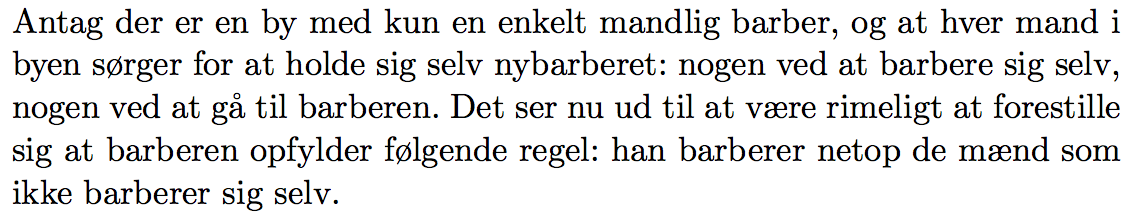
\includegraphics[width=0.8\textwidth]{opgD/barber.png}
        \label{fig:barber}
    \end{figure}
    
    Problemet med historien er; hvem barberer så barberen? \\
    Hvis barberen barberer sig selv, så må han ikke barbere sig selv; men hvis han ikke barberer sig selv, så barberer han sig selv.\\
    \\
    
    \item Analyse af barber problemet:
    
    Under den givne fortolkning $\mathcal{F}$ givet ved:
    
    \begin{figure}[H]
        \hspace{7 mm}
        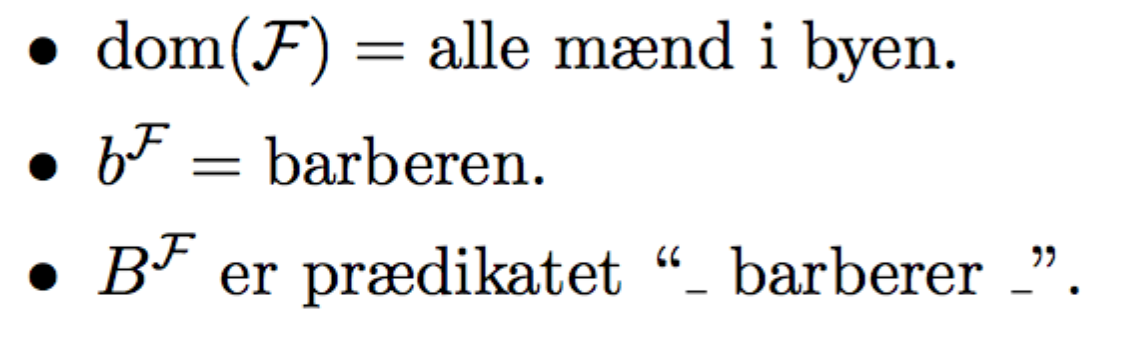
\includegraphics[width=0.4\textwidth]{opgD/barbFort.png}
        \label{fig:barbFort}
    \end{figure}
    
    Problemet bliver stilt op med med prædikationslogik som:
    
    \begin{equation*}
        \forall x (\neg B(x,x) \leftrightarrow B(b,x))
    \end{equation*}
    Udsagnet forstås som: "Barberen barberer dig, hvis og kun hvis du ikke barberer dig selv". Dette udsagns gyldighed kan kort tjekkes med tableau metoden:
    
     \[
 \begin{tikzpicture}[align=center,every edge quotes/.style={magenta,auto,font=\scriptsize}]
   \graph[trie,tree layout,level sep=7mm,sibling distance=30mm] 
   {

    "\formel{1}{\forall x (\neg B(x,x) \leftrightarrow B(b,x))}{T}" 
    -- 
    
    "\formel{2}{\neg B(b,b) \leftrightarrow B(b,b)}{T}"
    [> "$\allt$ på 1"] -- 
    
    {
        "\formel{3}{\neg B(b,b)}{T}\\
        \formel{4}{B(b,b)}{T}" -- "\formel{7}{B(b,b)}{F} \\ \times" [>"$\negt$ på 3"] ,
         "\formel{5}{\neg B(b,b)}{F}\\
        \formel{6}{B(b,b)}{F}" [>"$\leftrightarrow\T$ på 2"] -- "\formel{8}{B(b,b)}{T}  \\ \times" [>"$\negf$ på 5"]
    }
    
  };
  \end{tikzpicture}
\]

Alle grene bliver lukket. Udsagnet er derfor ikke opfyldeligt og dermed ikke gyldigt.
\end{enumerate}